% K80 model of evolution.
% A <--> G 	purines
% ^\   / ^
% |  X   |
% v/   \ v
% C <--> T	pyrimidines
%
% $ pdflatex k80
% $ pdf2svg k80.pdf k80.svg

\documentclass[11pt,tikz,border=2pt]{standalone}
\usepackage{tikz}
\usetikzlibrary{arrows,positioning}
\begin{document}
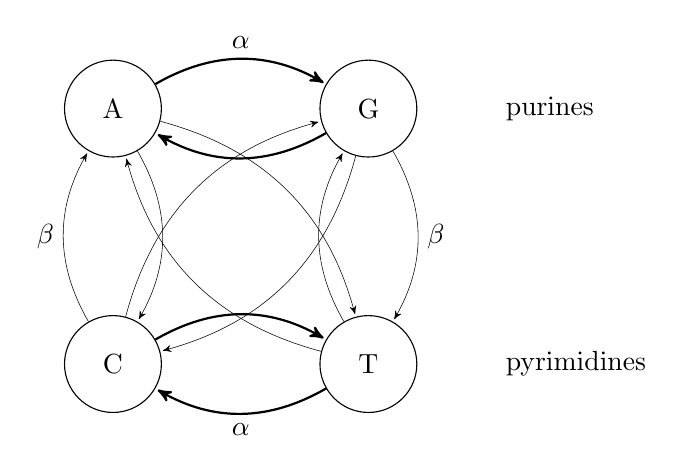
\begin{tikzpicture}[->,>=stealth',shorten >=1pt,auto,
		main node/.style={circle,draw,minimum size=35pt},
		ntclass node/.style={},
		invis node/.style={circle,minimum size=35pt}]
	\node[main node] (0) {A};
	\node[main node] (1) [right =2cm of 0] {G};
	\node[main node] (2) [below =2cm of 0] {C};
	\node[main node] (3) [right =2cm of 2] {T};
	\node[ntclass node] (100) [right =1cm of 1] {purines};
	\node[ntclass node] (101) [right =1cm of 3] {pyrimidines};
	%
	% Thick lines between purines A and G.
	\path[thick]
		(0) edge [bend left] node {$\alpha$} (1)
		(1) edge [bend left] node {} (0);
	%
	% Thick lines between pyrimidines C and T.
	\path[thick]
		(2) edge [bend left] node {} (3)
		(3) edge [bend left] node {$\alpha$} (2);
	%
	% Thin lines connecting a purine to a pyrimidine.
	\path[very thin]
		(0) edge [bend left] node {} (2)
		(2) edge [bend left] node {$\beta$} (0);
	\path[very thin]
		(1) edge [bend left] node {$\beta$} (3)
		(3) edge [bend left] node {} (1);
	\path[very thin]
		(0) edge [bend left] node {} (3)
		(3) edge [bend left] node {} (0);
	\path[very thin]
		(1) edge [bend left] node {} (2)
		(2) edge [bend left] node {} (1);
\end{tikzpicture}
\end{document}
